\chapter{Klassenbeschreibung Data Layer}

In diesem Kapitel werden die Klassen des Data Layers beschrieben, insbesondere die Repository-Klassen.

\section{Repository}

Das Repository bietet Zugriff zu den Datenquellen. Im Falle von Exzellenzkoch sind da die lokale SQLite Datenbank, zu welcher der Zugriff durch die Room Persistence Library gestellt wird, und der Webserver.
In diesem Kapitel soll es um das Modell der lokalen SQLite Datenbank gehen, der Webserver wird im Kapitel 9 behandelt.

\subsection{Modell für SQLite-Datenbank}

\begin{figure}[H]
\centering
\includegraphics[width=0.7\textwidth]{pics/AppSqLiteObjects.pdf}%
\caption{Klassendiagramm für das Model für die SQLite Datenbank in der App}%
\end{figure}

Das Diagramm zeigt Klassen die jeweils eine Tabelle von der SQLite Datenbank in der App abbilden. Diese Klassen werden in Verbindung mit DAOs, welche im folgenden Unterkapitel beschrieben werden, verwendet, um Daten von der SQLite Datenbank abzurufen. %Wenn die Datenbankanbindung mit Room realisiert wird, bekommen die Attribute bestimme Notifikation, welche 
Im folgenden werden diese Klassen genauer beschrieben:

Für die öffentlichen Rezepte werden die Klassen PublicRecipe, PublicRecipeTag, IngredientChapter und IngredientAmount verwendet.
Für die private Rezepte werden die Klasse PrivateRecipe und PrivateRecipeTag verwendet. Die Klasse ShoppingList ist für die Einkaufsliste und die PrivateTag für die private Tags, welche man erstellen kann.

\subsubsection{PublicRecipe}
Diese Klasse beschreibt ein öffentliches Rezept, welches von der Datenbank geladen oder gespeichert wird.

\textbf{Attribute}
\begin{itemize}
	\item <<get>>-recipeId:int\\Eindeutige Identifikation eines öffentlichen Rezeptes
	\item <<get/set>>-title:String\\Title eines Rezeptes
	\item <<get/set>>-ingredientsText:String\\Alle Zutaten als zusammenhängender Text
	\item <<get/set>>-preparationDescription\\Zubereitungsbeschreibung eines Rezeptes
	\item <<get/set>>-picture:BufferedImage\\Bild des Gerichts
	\item <<get/set>>-cookingTime:int\\Dauer für das Kochen
	\item <<get/set>>-preperationTime:int\\Dauer für die Zubereitung
	\item <<get>>-userId:String\\Id des Nutzers, dem das Rezept gehört
	\item <<get/set>>-creationDate:Date\\Das Datum an dem das Rezept erstellt wurde
	\item <<get/set>>-portions:int\\Anzahl für wie viel Personen das Rezept gedacht ist
\end{itemize}

\subsubsection{PublicRecipeTag}
Diese Klasse repräsentiert ein Tag für ein Rezept.

\textbf{Attribute}
\begin{itemize}
	\item <<get/set>>-tagId:String \\Name des Tags
	\item <<get/>>-recipeId:int \\Id des Rezeptes zu dem der Tag zugewiesen ist
\end{itemize}

\subsubsection{IngredientChapter}
Diese Klasse repräsentiert ein Kapitel von den Zutaten für ein Rezept.

\textbf{Attribute}
\begin{itemize}
	\item <<get>>-chapterId:int \\Die Id des Kapitels
	\item <<get>>-recipeId:int \\Die Id eines Rezeptes zu dem ein Kapitel zugewiesen ist
	\item <<get/set>>-ingredientChapterTitle:String \\Der Titel des Kapitels
\end{itemize}

\subsubsection{IngredientAmount}
Diese Klasse repräsentiert eine Zutat von einem Kapitel für ein Rezept.

\textbf{Attribute}
\begin{itemize}
	\item <<get>>-chapterId:int \\Id des Kapitels zu dem die Zutat zugeordnet ist
	\item <<get/set>>-nameIngredient:String \\Name der Zutat
	\item <<get/set>>-amount:int \\Menge der Zutat
	\item <<get/set>>-unit:String \\Einheit der Zutat
\end{itemize}

\subsubsection{PrivateTags}
Diese Klasse repräsentiert ein privates Tag, welches erstellt werden kann.

\textbf{Attribute}
\begin{itemize}
	\item <<get/set>>-tagId:String \\Name des privaten Tags
\end{itemize}

\subsubsection{ShoppingList}
Diese Klasse repräsentiert einen Eintrag in der Einkaufsliste.

\textbf{Attribute}
\begin{itemize}
	\item <<get>>-shoppingListId:int \\Eindeutiger Id für ein Einkaufslisteneintrag
	\item <<get/set>>-nameIngredient:String \\Name der Zutat
	\item <<get/set>>-amount:int \\Menge der Zutat
	\item <<get/set>>-unit:String \\Einheit der Zutat
\end{itemize}

\subsubsection{PrivateRecipe}
Diese Klasse repräsentiert ein privates Rezept.

\textbf{Attribute}
\begin{itemize}
	\item <<get>>-recipeId:int\\Eindeutige Identifikation eines öffentlichen Rezeptes
	\item <<get/set>>-title:String\\Title eines Rezeptes
	\item <<get/set>>-ingredientsText:String\\Alle Zutaten als zusammenhängender Text
	\item <<get/set>>-preparationDescription\\Zubereitungsbeschreibung eines Rezeptes
	\item <<get/set>>-picture:BufferedImage\\Bild des Gerichts
	\item <<get/set>>-cookingTime:int\\Dauer für das Kochen
	\item <<get/set>>-preperationTime:int\\Dauer für die Zubereitung
	\item <<get/set>>-creationDate:Date\\Das Datum an dem das Rezept erstellt wurde
	\item <<get/set>>-portions:int\\Anzahl für wie viel Personen das Rezept gedacht ist
\end{itemize}

\subsubsection{PrivateRecipeTag}
Diese Klasse repräsentiert ein Tag für ein Rezept.

\textbf{Attribute}
\begin{itemize}
	\item <<get/set>>-tagId:String \\Name des Tags
	\item <<get/>>-recipeId:int \\Id des Rezeptes zu dem der Tag zugewiesen ist
\end{itemize}

%DAOs
\subsection{Daoklassen für die Datenbank}
\subsubsection{DAO Entwurfsmuster}
Data Access Object (DAO) ist ein Entwurfsmuster, das den Zugriff auf unterschiedliche Arten von Datenquellen so kapselt, dass die angesprochene Datenquelle ausgetauscht werden kann, ohne dass der aufrufende Code geändert werden muss.
Dadurch soll die eigentliche Programmlogik von technischen Details der Datenspeicherung befreit werden und flexibler einsetzbar sein. DAO ist also ein Muster für die Gestaltung von Programmierschnittstellen (APIs). Diese Klassen bieten die Schnittstellen für den Zugriff auf die SQLite Datenbank.
\begin{figure}[H]
	\centering
	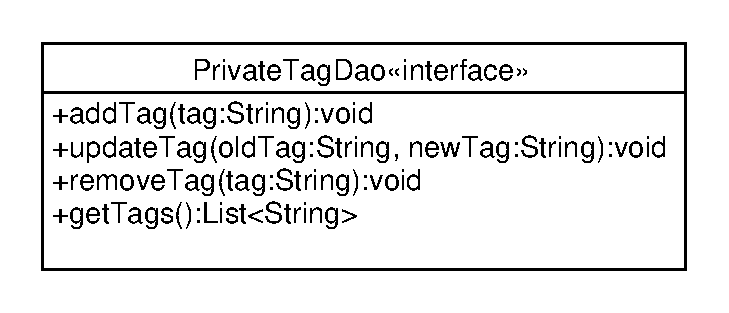
\includegraphics[width=0.7\textwidth]{pics/AppSqLiteDao.pdf}%
	\caption{Klassendiagramm für die Daos für die Sqlite Datenbank in der App}%
\end{figure}

\subsubsection{PublicRecipeDao<<interface>>}
Diese Klasse gibt Schnittstellen für das öffentliche Rezept in der Datenbank an.

\textbf{Methoden}
\begin{itemize}
	\item +addRecipe(recipe:PublicRecipe):void \\Fügt das übergebene neue Rezept hinzu
	\item +updateRecipe(recipe:PublicRecipe):void \\Aktualisiert einen Eintrag mit dem übergebenen Rezept
	\item +deleteRecipe(idRecipe:int):void \\Löscht ein Rezept mit der entsprechenden Id
	\item +getRecipe(idRecipe:int):PublicRecipe \\Gibt das Rezept mit der entsprechenden Id zurück
	\item +getRecipeChapter(idRecipe:int):List<IngredientChapter> \\Gibt die Kapitel des Rezeptes zurück
	\item +getTags(idRecipe:int):List<RecipeTag> \\Gibt die Tags eines Rezeptes zurück
	\item +addTag(recipeId:int, tagId:String):void \\Fügt ein Tag zu einem Rezept hinzu
	\item +removeTag(recipeId:int, tagId:String):void \\Entfernt ein Tag von einem Rezept
	\item +getFavourites():List<PublicRecipe> \\Gibt alle Favouriten vom Nutzer zurück
\end{itemize}

\subsubsection{IngredientChapterDao<<interface>>}
Diese Klasse gibt Schnittstellen für das Zutatenkapitel eines Rezeptes in der Datenbank an.

\textbf{Methoden}
\begin{itemize}
	\item +addChapter(chapter:IngredientChapter):void \\Fügt das übergebene Kapitel hinzu
	\item +editChapter(chapter:IngredientChapter):void \\Aktualisiert eine Kapitel mit dem übergebenen Kapitel
	\item +deleteChapter(idChapter:int):void \\Löscht ein Kapitel mit der entsprechenden Id
	\item +getIngredientAmount(idChapter:int):List<IngredientAmount> \\ Gibt die Liste von Zutaten von einem Kapitel zurück
	\item +getInregendientChapterFromRecipe(recipeId:int):List<IngredientChapter> \\Gibt die Liste an Kapitel von einem Rezept zurück
\end{itemize}

\subsubsection{IngredientAmountDao<<interface>>}
Diese Klasse gibt Schnittstellen für Zutaten eines Kapitels eines Rezeptes in der Datenbank an.

\textbf{Methoden}
\begin{itemize}
	\item +addIngredient(ingredient:IngredientAmount):void \\Fügt die übergeben Zutat hinzu
	\item +updateIngredient(ingredient:IngredientAmount):void \\Aktualisiert eine Zutat mit der übergeben Zutat
	\item +deleteIngredient(idChapter:int, nameIngredient:String):void \\Löscht eine Zutat mit der entsprechenden Kapitelid und Zutatennamen
\end{itemize}

\subsubsection{PrivateRecipeDao<<interface>>}
Diese Klasse gibt Schnittstellen für das private Rezept in der Datenbank an.

\textbf{Methoden}
\begin{itemize}
	\item +addRecipe(recipe:PublicRecipe):void \\Fügt das übergebene neue Rezept hinzu.
	\item +updateRecipe(recipe:PublicRecipe):void \\Aktualisiert einen Eintrag mit dem übergebenen Rezept
	\item +deleteRecipe(idRecipe:int):void \\Löscht ein Rezept mit der entsprechenden Id
	\item +getRecipe(idRecipe:int):PublicRecipe \\Gibt das Rezept mit der entsprechenden Id zurück
	\item +getTags(idRecipe:int):List<RecipeTag> \\Gibt die Tags eines Rezeptes zurück
	\item +addTag(recipeId:int, tagId:String):void \\Fügt ein Tag zu einem Rezept hinzu
	\item +removeTag(recipeId:int, tagId:String):void \\Entfernt ein Tag von einem Rezept
\end{itemize}

\subsubsection{ShoppingListDao<<interface>>}
Diese Klasse gibt Schnittstellen für die Einkaufsliste in der Datenbank an.

\textbf{Methoden}
\begin{itemize}
	\item +addShoppingList(item:ShoppingList):void \\Fügt das übergebene neue ShoppingListelement hinzu.
	\item +updateShoppingList(item:ShoppingList):void \\Aktualisiert ein ShoppingListelement mit dem übergebenen Element
	\item +deleteShoppingList(idShoppingList:int):void \\Löscht einen Eintrag in der ShoppingList mit der entsprechenden Id
	\item +getShoppingList():List<ShoppingList> \\Gibt die Einkaufsliste zurück
\end{itemize}

\subsubsection{PrivateTagDao<<interface>>}
Diese Klasse gibt Schnittstellen für die Einkaufsliste in der Datenbank an.

\textbf{Methoden}
\begin{itemize}
	\item +addTag(tag:String):void \\Fügt einen neuen privaten Tag hinzu
	\item +updateTag(oldTag:String, newTag:String):void \\Aktualisiert einen private Tag
	\item +removeTag(tag:String):void \\Löscht einen privaten Tag
	\item +getTags():List<String> \\Gibt alle privaten Tags zurück
\end{itemize}

\section{Datenbank}

\subsection{ClientDatenbank}

\begin{sidewaysfigure}[ht]
	\centering
	\includegraphics[width=1.0\textwidth]{pics/ClientDB.pdf}%
	\caption{ER-Diagramm der Clientdatenbank}%
\end{sidewaysfigure}

\textbf{Shoppinglist}\\
Die Relation ShoppingList beinhaltet Informationen über die Einkaufsliste.

\begin{itemize}
	\item shoppingListId \\ Id der eine ShoppingList-Eintrages
	\item nameIngrient \\ Name der Zutat
	\item unit \\ Einheit, in der die Zutat gemessen wird
	\item amount \\ Anzahl an unit in der die Zutat benötigt wird
\end{itemize}

\textbf{PublicRecipe}\\
Die Relation PublicRecipe beinhaltet Informationen über favoriserte Rezepte. Die Relation PublicRecipe wird über einen Fremdschlüssel in der Relation PublicRecipeTag und IngredientChapter adressiert und verweist selbst auf die Relation User.

\begin{itemize}
	\item recipeId \\ Eindeutige Kennung des Rezeptes in der Serverdatenbank (Primärschlüssel)
	\item title \\ Titel des Rezeptes
	\item ingredientsText \\ Textuelle Beschreibung der Zutaten
	\item preparationDescription \\ Textuelle Beschreibung der Zubereitung
	\item picture \\ Bild des Rezeptes
	\item cookingTime \\ Dauer der Kochzeit in Minuten
	\item preparationTime \\ Dauer der Vorbereitung in Minuten
	\item userId \\ Eindeutige Kennung des Ersteller des Rezeptes in der Serverdatenbank (Fremdschlüssel)
	\item creationDate \\ Datum und Uhrzeit der Veröffentlichung des Rezeptes
	\item portions \\ Anzahl Portionen für die das Rezept ausgelegt ist
\end{itemize}
%% soll wirklich der Text der Zutaten gespeichert werden? Den kann man doch ganz einfach aus den IngredientChapter und so berechnen,

\textbf{IngredientChapter}\\
Die Relation IngredientChapter beinhaltet Informationen über die Unterkapitel in der Zutatenliste. Die Relation IngredientChapter wird über einen Fremdschlüssel in der Relation IngredientAmount adressiert und verweist selbst auf die Relation PublicRecipe.

\begin{itemize}
	\item chapterId \\ Eindeutige Kennung des Unterkapitels (Primärschlüssel)
	\item recipeId \\ Zeiger auf das Rezept (Fremdschlüssel)
	\item ingredientChapterTitle \\Title des Chapters
\end{itemize}
% bin mir nicht ganz sicher was ingredientAmount ist, aber müsste nicht noch der Name des Kapitels gespeichert werden?

\textbf{IngredientAmount}\\
Die Relation IngredientAmount beinhaltet Informationen über die Zutaten in einem Unterkapitel einer Zutatenliste eines Rezeptes. Die Relation IngredientAmount verweist selbst auf die Relation IngredientChapter.

\begin{itemize}
	\item chapterId \\ Zeiger auf das Unterkapitel (Fremdschlüssel)
	\item nameIngredient \\ Name der Zutat
	\item unit \\ Einheit, in der die Zutat gemessen wird
	\item amount \\ Anzahl an unit in der die Zutat benötigt wird
\end{itemize}

\textbf{PublicRecipeTag}\\
Die Relation PublicRecipeTag beinhaltet Informationen über die Tags eines veröffentlichten Rezeptes. Die Relation PublicRecipeTag verweist auf die Relation PublicRecipe.

\begin{itemize}
	\item tagId \\ Name des Tags
	\item recipeId \\ Zeiger auf das Rezept (Fremdschlüssel)
\end{itemize}

\textbf{PrivateTags}\\
Die Relation PrivateTags listet alle privaten Tags auf.

\begin{itemize}
	\item tagId \\ Name des Tags (Primärschlüssel)
\end{itemize}

\textbf{PrivateRecipe}\\
Die Relation PrivateRecipe listet alle von dem Nutzer erstellten Rezepte auf. Die Relation PrivateRecipe wird über einen Fremdschlüssel in der Relation PrivateRecipeTag adressiert.

\begin{itemize}
	\item recipeId \\ Eindeutige Kennung des Rezeptes in dieser Tabelle (Primärschlüssel)
	\item title \\ Titel des Rezeptes
	\item ingredientsText \\ Textuelle Beschreibung der Zutaten
	\item preparationDescription \\ Textuelle Beschreibung der Zubereitung
	\item picture \\ Bild des Rezeptes
	\item cookingTime \\ Dauer der Kochzeit in Minuten
	\item preparationTime \\ Dauer der Vorbereitung in Minuten
	\item creationDate \\ Datum und Uhrzeit der Veröffentlichung des Rezeptes (null falls nicht veröffenlticht)
	\item portions \\ Anzahl Portionen für die das Rezept ausgelegt ist 
\end{itemize}

\textbf{PrivateRecipeTag}\\
Die Relation PrivateRecipeTag weist jedem Rezept eine Menge an Tags zu. Die Relation PrivateRecipeTag verweist selbst auf die Relation PrivateRecipe.

\begin{itemize}
	\item tagId \\ Name des Tags
	\item recipeId \\ Zeiger auf das Rezept
\end{itemize}

